\documentclass [tikz, border=12pt] {standalone}

\begin{document}
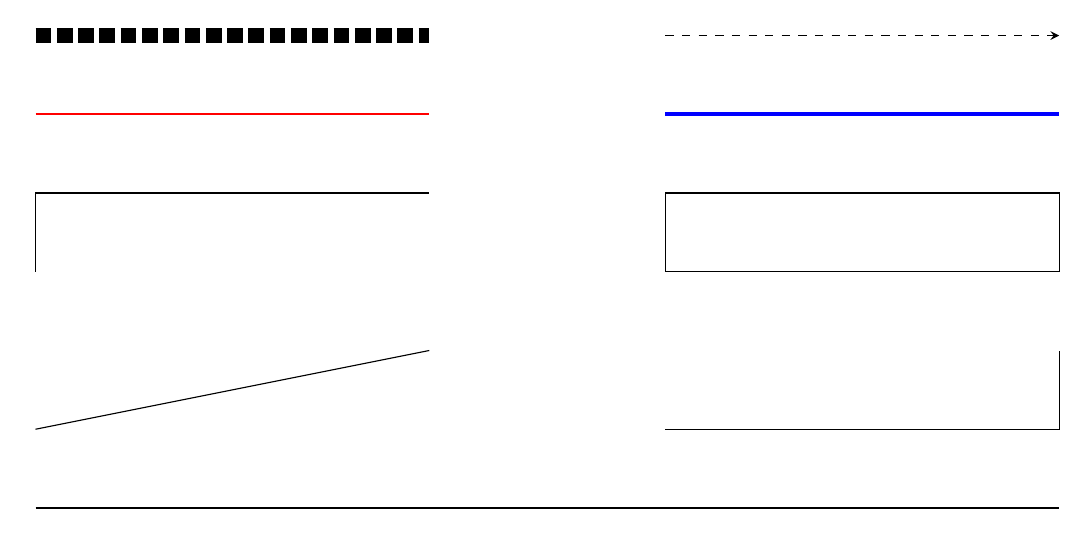
\begin{tikzpicture}

\draw (1,0)  -- (14,0); % 画一条线
\draw (1,1) to (6,2); % 画一条线
\draw (9,1) -| (14,2); % 画一条折线(先水平,后垂直)
\draw (1,3) |- (6,4) ; % 画一条折线(先垂直,后水平)
\draw (9,3) rectangle (14,4); % 画一个矩形
\draw [red,thick] (1,5) -- (6,5); % 红色,粗细:thick
\draw [blue,ultra thick] (9,5) -- (14,5); % 蓝色,粗细:ultra thick
\draw [dotted,line width=0.2cm] (1,6) -- (6,6); % 点线,粗细:0.2cm
\draw [dashed,->,>=stealth] (9,6) -- (14,6) ; % 虚线,端点形状:stealth箭头

\end{tikzpicture}
\end{document}
